\newpage
\begin{appendices}
\section{Evaluation of Existing Machine-learning based Name Generation Approaches for Generating Test Names}
\label[appendix]{sec:pilot-study}

Recent work has demonstrated that machine translation-based approaches can have significantly better performance than previous approaches in the context of generating identifiers and general method names (e.g.,~\cite{alon2018code2seq, alon2019code2vec}).
%
However, it is unknown how well these approaches work in the context of generating names for unit tests.
%
To evaluate their performance for this task, we conducted a pilot study.

\subsection{Considered Name Generations Approaches}

Work by \citeauthor{alon2018code2seq} is currently the state-of-the-art in using machine translation to generate names and identifiers based on source code~\cite{alon2018code2seq, alon2019code2vec}.
%
At a high-level, these approaches encode source code (e.g., methods) and labels (i.e., names) as a model that can be used to predict labels (names) for previously unseen inputs (code).
%
The primary difference between the approaches is that \texttt{Code2seq}~\cite{alon2018code2seq} encodes a source code as set of compositional paths while \texttt{Code2vec}~\cite{alon2019code2vec} encodes a source code as a fixed-length continuous vector.

\subsection{Considered Unit Tests}

\begin{table}[t]
\centering
\caption{Experimental Subjects.}
\begin{tabular}
{
  l
  l
  S[table-format=5.1]
  S[table-format=5.1]
}
\toprule
\multicolumn{1}{c}{\textbf{Project}} &
\multicolumn{1}{c}{\textbf{Version}} & 
\multicolumn{1}{c}{\textbf{LoC}} &
\multicolumn{1}{c}{\textbf{\# Tests}}
\\
\midrule
 Guice             & 9b371d3 &  183049  & 1280   \\
 Moshi             & dbed99d  &  22168  & 716   \\
 Picasso           & a087d26  &  11006  & 229  \\
 Fastjson          & e05f1f9  &  195511  & 4950   \\
 Guava             & 368c337  &  400801  & 13962  \\
 Mockito           & 22c82dc   &  59839 & 2145   \\
 Socket.io-client  & 661f1e7  &  9478  & 85  \\
 Scribejava        & ea42bc9  &  15184  & 110   \\
 ExoPlayer         & 79da521  &  172148  & 1510   \\
 Javapoet          & e9460b8  &  10755  & 302   \\
 Barbecue          & 44a8632  &  10760  & 170   \\
\bottomrule
\end{tabular}
\label{tab:subjectsForPilot}
\end{table}


To gather the tests we examined in our study, we started with the \num{11} Java projects shown in~\cref{tab:subjectsForPilot}.
%
In the table, the first column, \emph{Name}, shows the name of the project; the second column, \emph{Version}, shows the version of the project (either as a Git hash or version number); the fourth column, \emph{LoC}, shows the number of non-comment, non-blank lines of code as computed by SLOC count~\cite{nguyen2007sloc}; and the final column, \emph{\# Tests}, shows the number of unit tests in the project. In total, these \num{11} projects contain \num{25459} unit tests.
%
The first ten projects were randomly selected from the top \num{50} Java projects hosted on Github~\cite{top50projects}.
%
Because these projects encompass a variety of domains (e.g., JavaPoet is a library for generating Java programmatically and ExoPlayer is a media player for Android) and have many contributors (e.g., Moshi’s test suite contains contributions from \num{8} different people), their tests are more likely to be representative of tests in general which helps mitigate a potential threat to validity.
%
In addition, we also included Barbecue, a commonly used subject in the testing literature (e.g.,~\cite{zhang2015automatically, zhang2016towards, wu2020pattern}).


From these projects, we randomly selected \num{15400} tests.
%
The number of selected tests per project is proportional to the amount of tests in each project (i.e., more tests are selected from projects with more tests).
%
We tried our best to randomly choose various tests from different types of test classes that are written by different developers (e.g., judging by their commits).


\subsection{Data and Discussion}

To generate the data necessary for investigating the quality of the generated names, we ran \texttt{Code2seq} and \texttt{Code2vec} on the set of \num{15400} tests.
%
Both \texttt{Code2seq} and \texttt{Code2vec} were run on a MacBook Pro (2.4GHz Intel i5 processor and 8GB RAM) with MacOS Mojave \footnote{Same machine in the empirical study}, Tensorflow 1.13.1 and Tensorflow 2.0.0, respectively.
%
It took roughly \num{8} hours to both configure the necessary environment and to generate names for the tests.


\Cref{fig:duplicate-names} shows an example the names generated by both \texttt{Code2seq} and \texttt{Code2vec}.
%
\Cref{fig:generated1} shows two tests from Barbecue and the names generated for them using \texttt{Code2seq} and \cref{fig:generated2} shows two tests from ExoPlayer and the names generated for them using \texttt{Code2vec}.


\begin{figure}[H]
\centering
\begin{subfigure}[b]{1.0\textwidth}
\centering
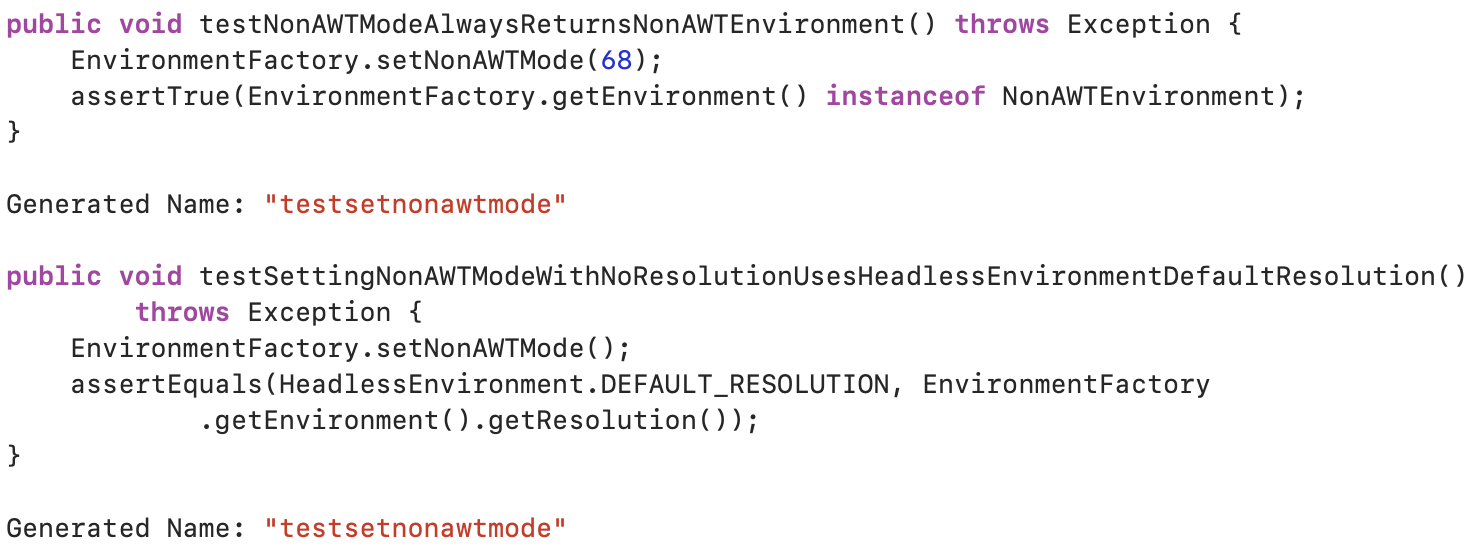
\includegraphics[scale=0.4]{figures/dup1.png}
\caption{Generated names by \texttt{Code2seq}.}
\label{fig:generated1}
\end{subfigure}\\
\vspace{0.2cm}
\begin{subfigure}[b]{1.0\textwidth}
\centering
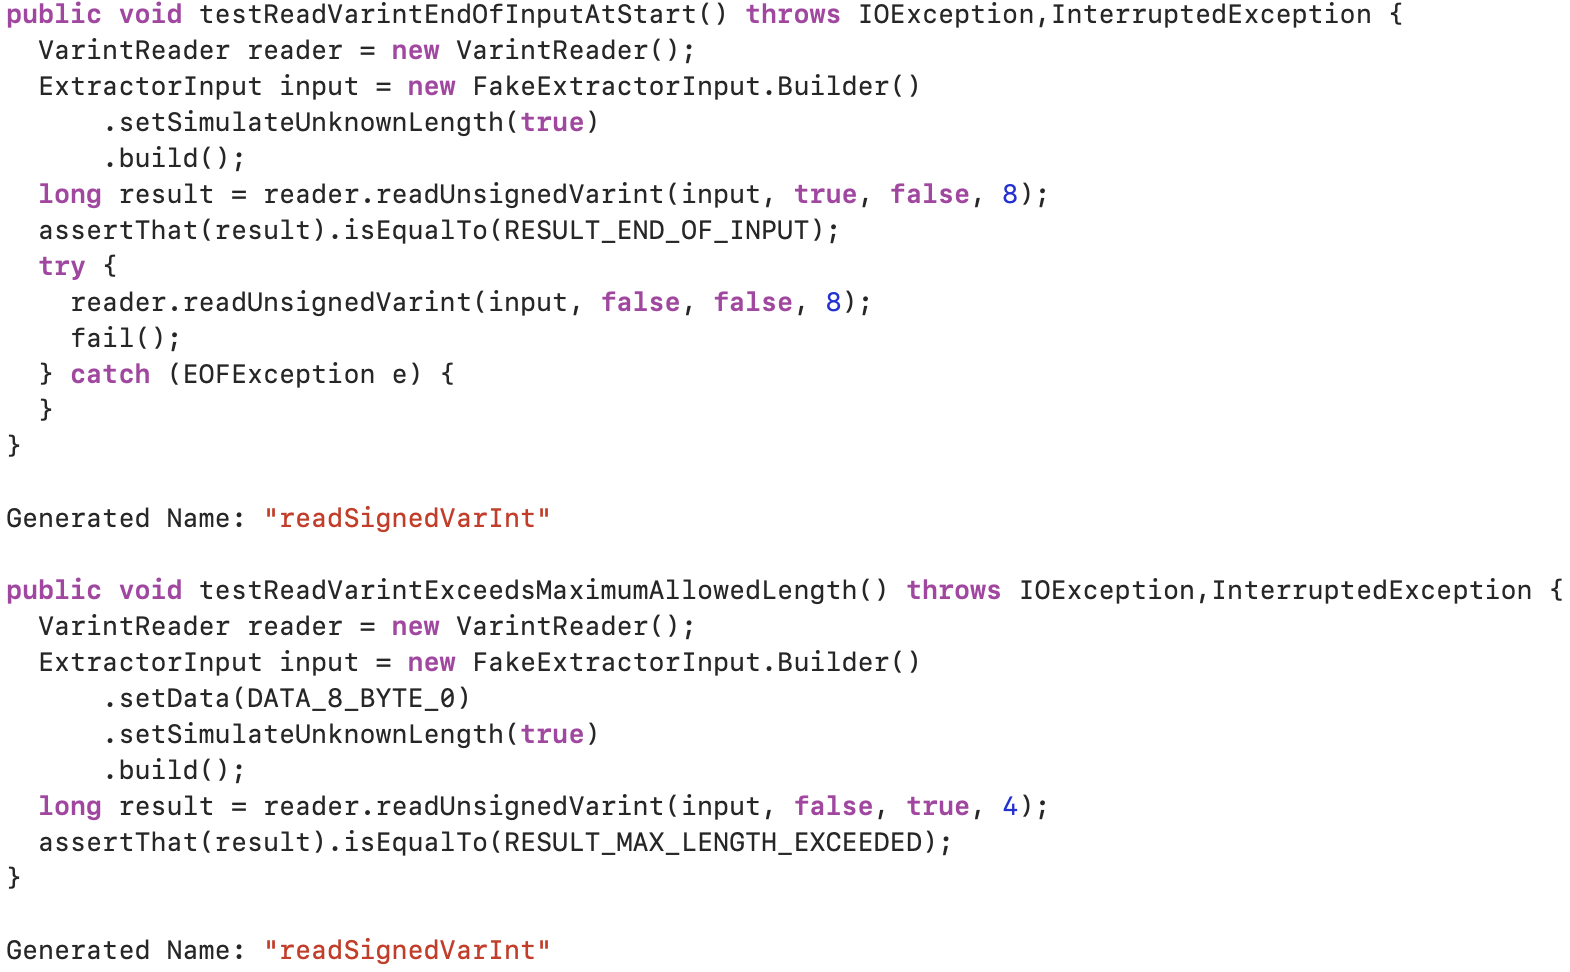
\includegraphics[scale=0.4]{figures/dup2.png}
\caption{Generated names by \texttt{Code2vec}.}
\label{fig:generated2}
\end{subfigure}
\caption{Example of generated names.}
\label{fig:duplicate-names}
\end{figure}


Initially, our manual assessment of the names was positive.
%
The names appeared to be descriptive at some level and were similar, module some capitalization, in format to existing test names.
%
However, we soon realized that both approaches frequently generated duplicate names for different tests in the same class.
%
For example, as shown in \cref{fig:generated1,fig:generated2}, both \texttt{Code2seq} and \texttt{Code2vec} generated the same name for different tests.


\begin{table}[t]
\centering
\caption{Collected Data for \texttt{Code2seq} and \texttt{Code2vec}.}
\begin{tabular}
{
  l
  S[table-format=5.1]
  S[table-format=3.1]
  S[table-format=5.1]
  S[table-format=3.1]
}
 
%TODO[fixed]: I'd like to see the percentage of duplicates.  You should add this as another column or in ().

\toprule
 & \multicolumn{4}{c}{\textbf{\# Duplicates}} \\
 \cmidrule(lr){2-5}
 
\multicolumn{1}{c}{\textbf{Project}} &
\multicolumn{1}{c}{\textbf{\texttt{Code2seq}}} & \multicolumn{1}{c}{\textbf{(\%)}} &
\multicolumn{1}{c}{\textbf{\texttt{Code2vec}}} &
\multicolumn{1}{c}{\textbf{(\%)}}
\\
\midrule
 Guice             &  174   & 14.4 & 195  &  14.8 \\
 Moshi             &  80    & 14.5 & 98   &  17.6  \\
 Picasso           &  48    & 14.1 & 50   &  14.7 \\
 Fastjson          &  256   & 14.2 & 258  &  14.4 \\
 Guava             &  1152  & 15.9 & 1161 &  16.2 \\
 Mockito           &  254   & 12.0 & 328  &  15.5 \\
 Socket.io-client  &  15    & 19.0 & 15   &  17.4 \\
 Scribejava        &  17    & 15.7 & 22   &  20.2 \\
 ExoPlayer         &  240   & 16.7 & 257  &  17.6 \\
 Javapoet          &  46    & 14.5 & 52   &  15.9 \\
 Barbecue          &  30    & 18.9 & 18   &  14.5 \\
\bottomrule
\end{tabular}
\label{tab:ml-approach-data}
\end{table}

\cref{tab:ml-approach-data} shows the extent of the duplication in our considered subjects.
%
The \emph{\# Duplicates} columns shows how many times the respective approach generated a duplicate name for tests in the same test class.
%
For example, the first row shows that, for Guice, \texttt{Code2seq} produced \num{174} duplicates and \texttt{Code2vec} produced \num{195} duplicates.
% TODO[fixed]: Update to match data.
As this data shows, duplication occurs in all of our considered subjects.
%
Moreover, it is common with up to \SI{\approx 14.5}{\percent} percent of tests having a duplicate name in Javapoet from \texttt{Code2seq} and \SI{\approx 15.9}{\percent} percent from \texttt{Code2vec}.


Because of the extent of the duplication issue, we believe that machine translation-based approaches are unlikely to be useful for generating names for unit tests without significant modification.

\end{appendices}